\documentclass{beamer}
%
% Choose how your presentation looks.
%
% For more themes, color themes and font themes, see:
% http://deic.uab.es/~iblanes/beamer_gallery/index_by_theme.html
%
\usepackage{graphicx}
\usepackage{graphics}
\mode<presentation>
{
  \usetheme{Madrid}      % or try Darmstadt, Madrid, Warsaw, default...
  \usecolortheme{crane} % or try albatross, beaver, crane, ...
  \usefonttheme{serif}  % or try serif, structurebold, ...
  \setbeamertemplate{navigation symbols}{}
  \setbeamertemplate{caption}[numbered]
} 

\usepackage[spanish]{babel}
\usepackage[utf8]{inputenc}
\usepackage[T1]{fontenc}

\title[Covid 19]{Covid 2019}
\author{Lenin G.F.}
\institute{E.P.N}
\date{\today}

\begin{document}

\begin{frame}
  \titlepage
\end{frame}

% Uncomment these lines for an automatically generated outline.
\begin{frame}{Outline}
 \tableofcontents
\end{frame}

\section{Introducción}
\begin{frame}{Modelando Pandemias}
    \begin{itemize}
        \item<1-> La pandemia es una función exponencial.
        \item<2-> Existen modelos antiguos como el SIR.
        \item<3-> Otros virus son SarsCov1. 
    \end{itemize}
\end{frame}
\usebackgroundtemplate%
{%
    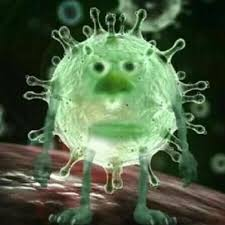
\includegraphics[width=\paperwidth,height=\paperheight]{figuras/covid.jpeg}%
}
\begin{frame}{Foto de un Corona Virus}
    \centering
    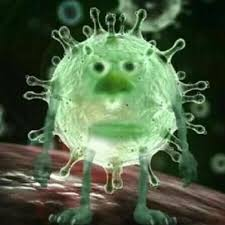
\includegraphics[width=\textwidth]{figuras/covid.jpeg}\\
    % Este es el Corona Virus que ha causado miles de muertes en unos pocos meses desde diciembre 2019
\end{frame}

\section{Metodología}
\begin{frame}{Materiales y Métodos}
    \begin{itemize}
        \item Recolección de muestras de esputo.
        \item Sintetizar ARN de muestras
        \item Determinar si el candidato es positivo o negativo
    \end{itemize}
    
    El teorema de Pitágoras es : $z^2 = x^2 +y^2$
    La teoría de la relatividad es:
    \begin{equation*}
        E = mc^2    
    \end{equation*}

\end{frame}
\usebackgroundtemplate{}
\section{Experimentos}
\begin{frame}{Experiimentos Realizados}
    Describir experimentos
\end{frame}

\section{Conclusiones}
\begin{frame}{Conclusiones}
    Poner las conclusiones
\end{frame}
\end{document}
